\chapter{Modèle conceptuel des données}

\section{Introduction}

\subsection{Objectifs du document}

Cette section sert à documenter et valider les éléments persistants qui devront
être stockés dans le système informatique de la gestion de calendriers de médecins.

\subsection{Domaine de définition du document}

Cette section reprend la description du diagramme métier (diagramme de classes) de la gestion de 
calendriers de médecins.

\subsection{Définitions, acronymes et abréviations}

\begin{enumerate}

\item \texttt{INAMI} : Institut national d'assurance maladie invalidité.

\end{enumerate}

\subsection{Références}

Énoncé du travail de synthèse sur la gestion de calendriers de médecins.

\subsection{Domaine du projet global}
\newpage
\section{Diagramme(s) de classe(s)}

\begin{figure}[hb]
    \centering
    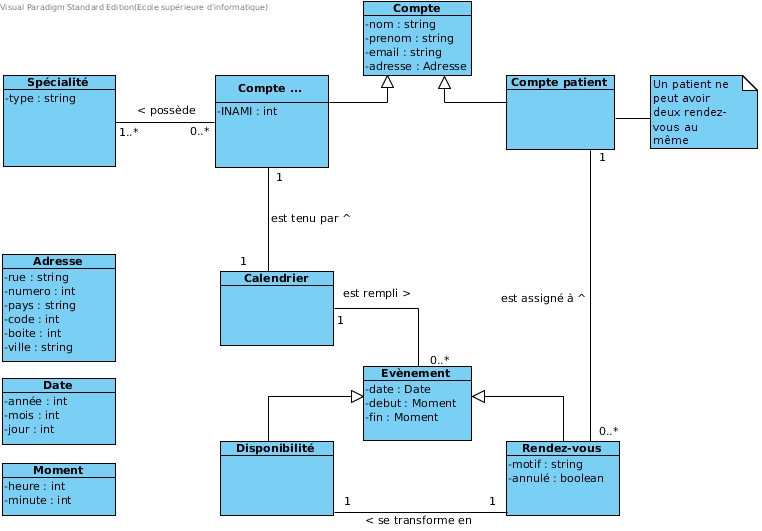
\includegraphics[scale=0.4]{MCD/MCD.jpg}
    \caption{Diagramme de classes Medicagenda}
\end{figure}

\newpage
\section{Classe(s)}


\subsection{Adresse}

\subsubsection{Définition}

Une adresse représente l'adresse postale d'une personne physique.

\subsubsection{Identifiant}

Tous les attributs d'une adresse forment un identifiant.

\subsubsection{Attributs}

\begin{itemize}
    \item rue
    \item numéro
    \item ville
    \item pays
    \item code (= code postal)
    \item boite (optionnel)
\end{itemize}

\subsubsection{Contraintes d'intégrité}

Aucune.

\subsection{Calendrier}

\subsubsection{Définition}

Le calendrier représente tous les évènements futurs et permet
au médecin d'organiser ces évènements. \\
Un client peut ajouter un rendez-vous au calendrier d'un médecin.

\subsubsection{Identifiant}

Médecin.INAMI

\subsubsection{Attributs}

Aucun.

\subsubsection{Contraintes d'intégrité}

Aucune.

\subsubsection{Condition de création / suppression d'un objet ou de la classe}

A la création d'un compte médecin, un calendrier est créé pour ce médecin. 
Il n'est pas supprimé.


\subsection{Compte}

\subsubsection{Définition}

Un compte représente un compte sur le site en ligne. Un compte permet la gestion 
d'un calendrier ainsi que des paramètres personnels du client. \\
\texttt{Compte} est la super classe\footnote{selon le principe d'héritage de
l'Orienté Objet} de \texttt{Compte client} et \texttt{Compte Médecin}. 

\subsubsection{Identifiant}

Compte.e-mail

\subsubsection{Attributs}

\begin{itemize}
    \item Nom
    \item Prénom
    \item E-mail
    \item Adresse
\end{itemize}

\subsubsection{Contraintes d'intégrité}

Aucune.

\subsubsection{Condition de création / suppression d'un objet ou de la classe}

Un compte est créé par un médecin pour un client, ou par un médecin pour lui-même
ou par un client pour lui-même.
Une fois créé, il n'y a pas de possibilité de suppression.


\subsection{Compte médecin}

\subsubsection{Définition}

Un compte médecin est un type de compte permettant au médecin de gérer ses rendez-vous et disponibilités
grâce au \texttt{calendrier}.

\subsubsection{Identifiant}

Identifiant de \texttt{Compte}.

\subsubsection{Attributs}

Attributs de \texttt{Compte}.

\subsubsection{Contraintes d'intégrité}

Aucune.

\subsubsection{Condition de création / suppression d'un objet ou de la classe}

Voir \texttt{Compte}.

\subsection{Compte patient}

\subsubsection{Définition}

Un compte client est un type de compte permettant au client d'ajouter des rendez-vous avec un médecin.
Un client peut modifier ses paramètres dans son espace client.

\subsubsection{Identifiant}

Identifiant de \texttt{Compte}.

\subsubsection{Attributs}

Attributs de \texttt{Compte}.

\subsubsection{Contraintes d'intégrité}

Aucune.

\subsubsection{Condition de création / suppression d'un objet ou de la classe}

Voir \texttt{Compte}.

\subsection{Date}

\subsubsection{Définition}

Une date représente une date représentée par un jour, un mois et une année.

\subsubsection{Identifiant}

Date.jour + Date.mois + Date.année

\subsubsection{Attributs}

\begin{itemize}

    \item{jour}
    \item{mois}
    \item{année}

\end{itemize}

\subsubsection{Contraintes d'intégrité}

\begin{itemize}
    \item Un jour prend les valeurs entre 1 et 31.
    \item Un mois prend les valeurs entre 1 et 12.
    \item La valeur maximale du jour dépend du mois (30 / 31 / 28 / 28).
\end{itemize}

\subsubsection{Condition de création / suppression d'un objet ou de la classe}

\subsection{Disponibilité}

\subsubsection{Définition}

Une disponibilité est une plage horaire dans laquelle un médecin accepte
des nouveaux rendez-vous.

\subsubsection{Identifiant}

Événement.date + Événement.début + Événement.fin

\subsubsection{Attributs}

Voir \texttt{Événement}.

\subsubsection{Contraintes d'intégrité}

Voir \texttt{Événement}.

\subsubsection{Condition de création / suppression d'un objet ou de la classe}

Une disponibilité est créé lorsqu'un médecin décide d'accepter de nouveaux rendez-vous ou quand un
rendez-vous a été annulé par un client. Dans ce cas, le rendez-vous est transformé en disponibilité.

\subsection{Événement}

\subsubsection{Définition}

Un évènement est un horaire pendant lequel le médecin peut recevoir un patient ou en accepter de nouveaux.

\subsubsection{Identifiant}

Événement.date + Événement.début + Événement.fin

\subsubsection{Attributs}

\begin{itemize}
    \item date
    \item début
    \item fin
\end{itemize}

\texttt{début} et \texttt{fin} représentent des heures/minutes de début et fin d'un évènement.

\subsubsection{Contraintes d'intégrité}

$fin > début$.

\subsubsection{Condition de création / suppression d'un objet ou de la classe}

Un évènement est soit créé par un médecin, soit par un client. Une fois l'évènement passé,
il est stocké dans la base de données.

\subsection{Moment}

\subsubsection{Définition}

Un moment est représenté par une heure et des minutes.

\subsubsection{Identifiant}

Moment.heure + Moment.minute

\subsubsection{Attributs}

\begin{itemize}
    \item{heure}
    \item{minute}
\end{itemize}

\subsubsection{Contraintes d'intégrité}

\begin{itemize}
    \item heure doit être compris entre 0 et 23.
    \item minute doit être compris entre 0 et 59.
\end{itemize}

\subsubsection{Condition de création / suppression d'un objet ou de la classe}

\subsection{Rendez-vous}

\subsubsection{Définition}

Un rendez-vous est un horaire créé par le client ou par le médecin où le client se doit 
d'assister à la séance.
Un rendez-vous peut être annulé avant la date de ce dernier par le client lui-même.

\subsubsection{Identifiant}

Événement.date + Événement.début + Événement.fin

\subsubsection{Attributs}

\begin{itemize}
    \item motif
    \item annulé
\end{itemize}

\subsubsection{Contraintes d'intégrité}

Aucune

\subsubsection{Condition de création / suppression d'un objet ou de la classe}

Un rendez-vous est créé soit par le médecin, soit par le client. Il n'est jamais supprimé.

\subsection{Spécialité}

\subsubsection{Définition}

Une spécialité définit le type d'activité médicale qu'effectue le médecin.

\subsubsection{Identifiant}

Spécialité.type

\subsubsection{Attributs}

\begin{itemize}
    \item type
\end{itemize}

\subsubsection{Contraintes d'intégrité}

Aucune.

\newpage
\section{Associations}

\subsection{Association\_possède \texttt{Compte médecin-> Spécialité}}
\subsubsection{Définition}
Associe des spécialités à un médecin par le biais de son compte.
\subsubsection{Contraintes d'intégrité}
Le médecin ne peut posséder deux fois la même spécialité.

\subsection{Association\_tient un \texttt{Compte médecin -> Calendrier}}
\subsubsection{Définition}
Associe un calendrier de disponibilités à un médecin.
\subsubsection{Contraintes d'intégrité}
Il pourrait éventuellement cumuler plusieurs calendrier pour subdiviser ses
rendez-vous.

\subsection{Association\_est assigné à \texttt{Rendez-vous -> Compte patient}}
\subsubsection{Définition}
Associe un patient à un rendez-vous.
\subsubsection{Contraintes d'intégrité}
Un patient peut cumuler plusieurs rendez-vous mais jamais au même moment.

\subsection{Association\_est rempli de \texttt{Calendrier -> Événement}}
\subsubsection{Définition}
Associe un calendrier à des évènements qui le composent.
\subsubsection{Contraintes d'intégrité}
\texttt{Aucune}

\subsection{Association\_Se transforme en \texttt{Disponibilité -> Rendez-vous}}
\subsubsection{Définition}
Associe une disponibilité entant que rendez-vous.
\subsubsection{Contraintes d'intégrité}
Cette association peut être brisée.
\newpage

\section{Dictionnaire des données}

\begin{center}
\begin{longtable}{|p{2cm}|p{2cm}|p{3cm}|p{2cm}|p{2cm}|p{2cm}|}
		\hline
		Nom & Classe & Définition & Type & Domaine & CI \\
		\hline
		annulé & Rendez-vous & \parbox[t]{3cm}{Vrai si le rendez-vous a été annulé\\} &
        Booléen & Vrai ou faux & Aucune \\
		\hline
        adresse & Compte & \parbox[t]{3cm}{L'adresse du titulaire du compte\\} & Chaîne 
        & \parbox[t]{2cm}{Toutes adresses valables\\} & Aucune \\
        \hline
        année & Date & L'année de la date & Entier & \parbox[t]{2cm}{Aucun\\ domaine particulier\\} & Aucune \\
        \hline
        boite & Adresse & \parbox[t]{3cm}{Le numéro de la boîte postale\\} & Entier & \parbox[t]{2cm}{Aucun\\ domaine particulier\\} &
        Optionnel \\
        \hline
        code & Adresse & \parbox[t]{3cm}{Le code postal\\} & Entier & \parbox[t]{2cm}{Aucun\\ domaine particulier\\} & Aucune \\
        \hline
        date & Événement & \parbox[t]{3cm}{La date de l'évènement\\} & Date & \parbox[t]{2cm}{Aucun\\ domaine particulier\\} &
        Aucune \\
        \hline
        début & Événement & \parbox[t]{3cm}{L'heure de début de l'évènement\\} & Moment & \parbox[t]{2cm}{Aucun\\ domaine particulier\\} &
        Aucune \\
        \hline
        e-mail & Compte & \parbox[t]{3cm}{L'e-mail du titulaire du compte\\} & Chaîne & \parbox[t]{2cm}{Aucun\\ domaine particulier\\}
        & \parbox[t]{2cm}{E-Mail\\ valide} \\
        \hline
        fin & Événement & \parbox[t]{3cm}{L'heure de fin de l'évènement\\} & Moment & \parbox[t]{2cm}{Aucun\\ domaine particulier\\} &
        Aucune \\
        \hline
        heure & Moment & \parbox[t]{3cm}{L'heure du\\moment\\} & Entier & Valeur de 0 à 23 &
        Aucune \\
        \hline
        INAMI & Compte médecin & \parbox[t]{3cm}{Le numéro \\INAMI du médecin\\} & Entier & \parbox[t]{2cm}{Aucun\\ domaine particulier\\}
        & Aucune \\
        \hline
        jour & Date & Le jour de la date & Entier & 1 à 31 & \parbox[t]{2cm}{Valeur \\correcte du jour selon\\ le mois\\} \\
        \hline
        minute & Moment & \parbox[t]{3cm}{La minute de\\ l'heure du\\ moment\\} & Entier & Valeur de 0 à 59 &
        Aucune \\
        \hline
        mois & Date & Le mois de la date & Entier & Valeur de 1 à 12 & Aucune \\
        \hline
        motif & Rendez-vous & \parbox[t]{3cm}{Le motif \\du rendez-vous\\} & Chaîne & \parbox[t]{2cm}{Aucun\\ domaine particulier\\}
        & Aucune \\
        \hline
        nom & Compte & \parbox[t]{3cm}{Le nom du titulaire du compte\\} & Chaîne & \parbox[t]{2cm}{Aucun\\ domaine particulier\\}
        & Aucune \\
        \hline
        numéro & Adresse & \parbox[t]{3cm}{Le numéro dans la rue\\} & Entier & \parbox[t]{2cm}{Nombres positifs} & Aucune \\
        \hline
        pays & Adresse & \parbox[t]{3cm}{Le pays dans\\lequel se situe\\l'adresse\\}  & Chaîne & \parbox[t]{2cm}{Aucun\\ domaine particulier\\}  
        & Aucune \\
        \hline
        prénom & Compte & \parbox[t]{3cm}{Le prénom du titulaire du compte\\} & Chaîne & \parbox[t]{2cm}{Aucun\\ domaine particulier\\}
        & Aucune \\
        \hline
        rue & Adresse & \parbox[t]{3cm}{La rue de\\ l'adresse\\} & Chaîne & \parbox[t]{2cm}{Aucun\\ domaine particulier\\} & Aucune \\
        \hline
        type & Spécialité & \parbox[t]{3cm}{Le type de\\ la spécialité\\} & Chaîne & \parbox[t]{2cm}{Les types\\ valables\\} & Aucune\\
        \hline
        ville & Adresse & \parbox[t]{3cm}{La ville de\\ l'adresse\\} & Chaîne & \parbox[t]{2cm}{Aucun\\ domaine particulier\\} & Aucune \\
        \hline
        
\end{longtable}
\end{center}


